\section{Results}

\subsection{Quality evaluation}

Figure \ref{fig:0.1-MultiQC_FastQC_status_checks} shows an overview of the Trimmomatic\index{Trimmomatic} preprocessing (the surviving reads), created by MultiQC\index{MultiQC}.

\begin{figure}[htbp]
    \caption{Trimmomatic preprocessing}
    \label{fig:0.1-MultiQC_FastQC_status_checks}
    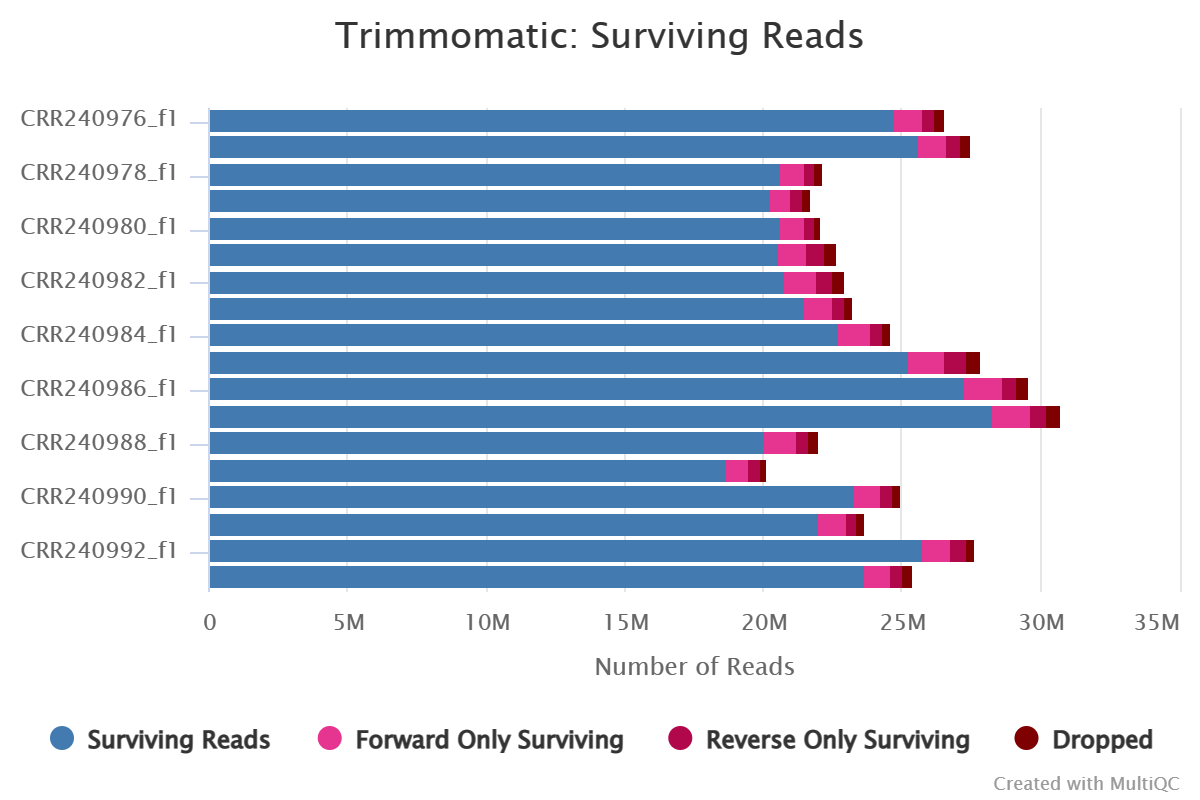
\includegraphics[width=0.75\textwidth]{../../results/multiqc/Plot-Exports/trimmomatic-surviving_reads}
\end{figure}

Figure \ref{fig:0.2-MultiQC_FastQC_status_checks} shows a MultiQC overview of the FastQC\index{FastQC} quality assessment of the trimmed FASTQ files.

\begin{figure}[htbp]
    \caption{FastQC quality assessment of the preprocessed FASTQ files}
    \label{fig:0.2-MultiQC_FastQC_status_checks}
    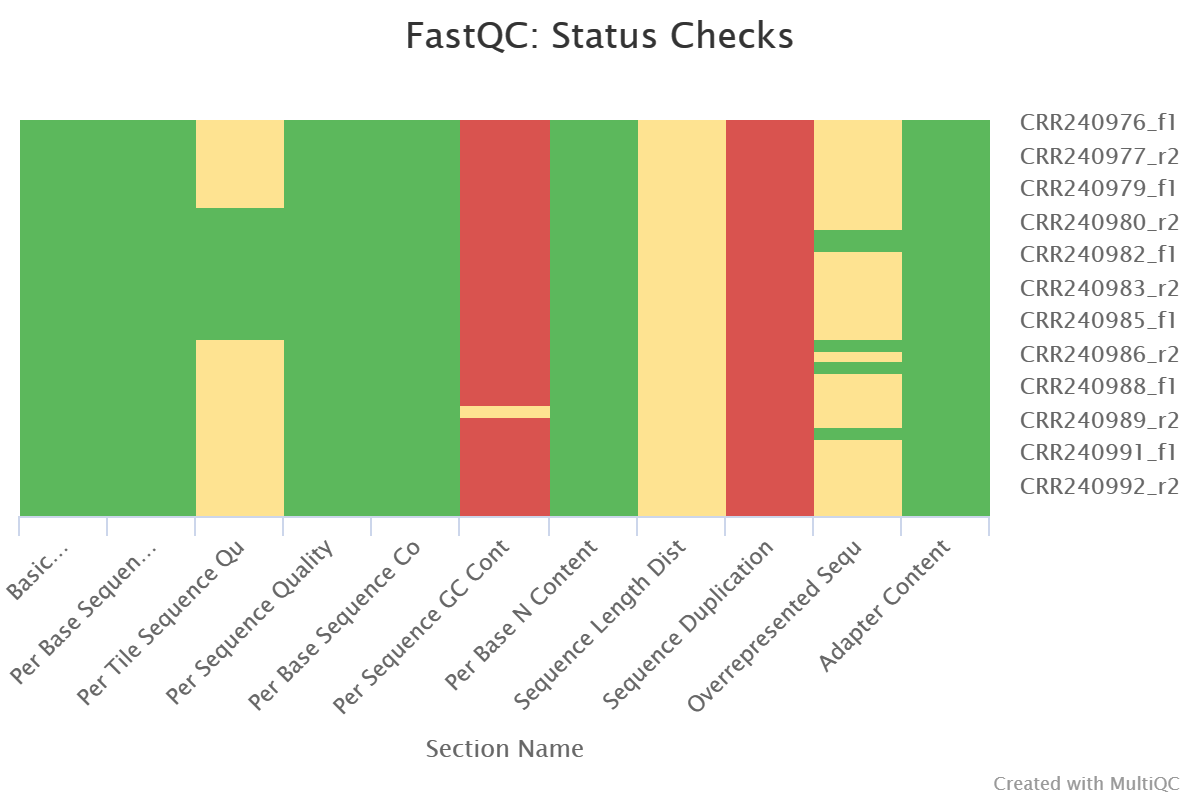
\includegraphics[width=0.75\textwidth]{../../results/multiqc/Plot-Exports/fastqc-status-check-heatmap}
\end{figure}

According to this quality assessment, the (trimmed) RNA-seq data may be regarded as good quality for the purpose of this research.


\subsection{Reads mapped to the reference transcriptome}

For most of the FASTQ files, kallisto pseudoaligned well above \qty{80}{\percent} of the (preprocessed) RNA-seq reads. Figure \ref{fig:0.3-MultiQC_kallisto_alignment} shows a MultiQC overview of the kallisto\index{kallisto} pseudoalignments.

\begin{figure}[htbp]
    \caption{kallisto pseudoalignments}
    \label{fig:0.3-MultiQC_kallisto_alignment}
    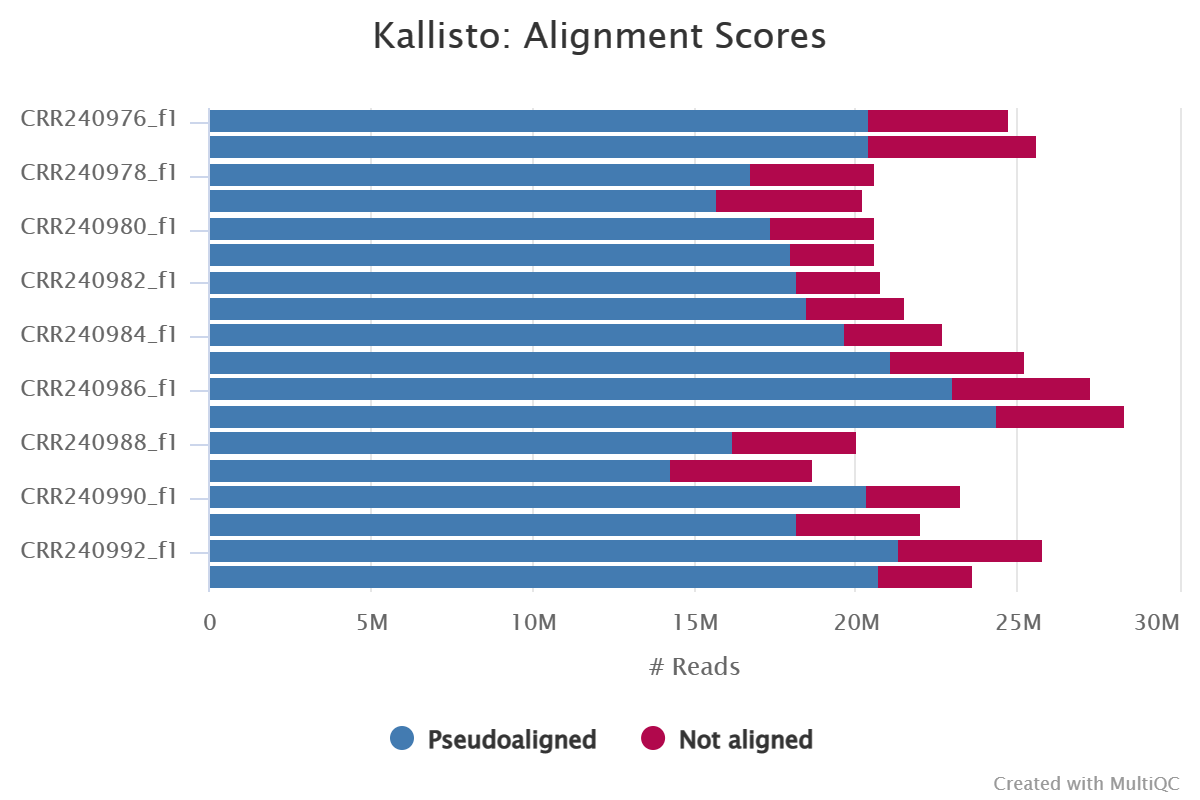
\includegraphics[width=0.75\textwidth]{../../results/multiqc/Plot-Exports/kallisto_alignment}
\end{figure}


\subsection{Exploratory data analysis}
Discuss the dominating variance components, reproducibility, possible batch effects and confounding variables.

\subsection{Differentially expressed genes}
Discuss the identified differentially expressed genes and their potential biological significance.

\subsection{Functional enrichment analysis}
Present the results of the functional enrichment analysis, highlighting the enriched functional categories.